% !TEX TS-program = pdflatex
% !TEX encoding = UTF-8 Unicode

% This is a simple template for a LaTeX document using the "article" class.
% See "book", "report", "letter" for other types of document.

\documentclass[11pt]{article} % use larger type; default would be 10pt

\usepackage{polski}
\usepackage[utf8]{inputenc} % set input encoding (not needed with XeLaTeX)
\usepackage{float}
\usepackage{tabto}

%%% Examples of Article customizations
% These packages are optional, depending whether you want the features they provide.
% See the LaTeX Companion or other references for full information.

%%% PAGE DIMENSIONS
\usepackage{geometry} % to change the page dimensions
\geometry{a4paper} % or letterpaper (US) or a5paper or....
% \geometry{margin=2in} % for example, change the margins to 2 inches all round
% \geometry{landscape} % set up the page for landscape
%   read geometry.pdf for detailed page layout information

\usepackage{graphicx} % support the \includegraphics command and options
\graphicspath{ {./images/} }

% \usepackage[parfill]{parskip} % Activate to begin paragraphs with an empty line rather than an indent

%%% PACKAGES
\usepackage{booktabs} % for much better looking tables
\usepackage{array} % for better arrays (eg matrices) in maths
\usepackage{paralist} % very flexible & customisable lists (eg. enumerate/itemize, etc.)
\usepackage{verbatim} % adds environment for commenting out blocks of text & for better verbatim
\usepackage{subfig} % make it possible to include more than one captioned figure/table in a single float
% These packages are all incorporated in the memoir class to one degree or another...

%%% HEADERS & FOOTERS
\usepackage{fancyhdr} % This should be set AFTER setting up the page geometry
\pagestyle{fancy} % options: empty , plain , fancy
\renewcommand{\headrulewidth}{0pt} % customise the layout...
\lhead{}\chead{}\rhead{}
\lfoot{}\cfoot{\thepage}\rfoot{}

%%% SECTION TITLE APPEARANCE
\usepackage{sectsty}
\allsectionsfont{\sffamily\mdseries\upshape} % (See the fntguide.pdf for font help)
% (This matches ConTeXt defaults)

%%% ToC (table of contents) APPEARANCE
\usepackage[nottoc,notlof,notlot]{tocbibind} % Put the bibliography in the ToC
\usepackage[titles,subfigure]{tocloft} % Alter the style of the Table of Contents
\renewcommand{\cftsecfont}{\rmfamily\mdseries\upshape}
\renewcommand{\cftsecpagefont}{\rmfamily\mdseries\upshape} % No bold!

%%% END Article customizations

%%% The "real" document content comes below...

\title{Stacja pogodowa w oparciu o system operacyjny czasu rzeczywistego Zephyr oraz płytę prototypową Arduino Nano 33 BLE}
\author{%
   Mateusz Matkowski (145432) \and 
   Mikołaj Starzak (158958)}

\begin{document}
\maketitle

\section{Wprowadzenie}

Projekt związany jest z wykorzystaniem systemu Zephyr do pomiaru i prezentacji danych z czujnika temperatury i ciśnienia. Aplikacja powinna działać w oparciu o system Zephyr oraz płytę prototypową Arduino Nano 33 BLE.

\section{Wykorzystane technologie}

\subsection{Sprzęt}

\begin{itemize}
\item Arduino Nano 33 BLE,
\item BMP280 - czujnik ciśnienia i temperatury,
\item Telefon z Androidem.
\item Komputer z USB.
\end{itemize}

\subsection{Oprogramowanie i protokoły}

\begin{itemize}
\item Zephyr - system operacyjny czasu rzeczywistego,
\item nRF Connect - mobilna aplikacja do zarządzania połączeniami Bluetooth na telefonach,
\item I2C - protokół do komunikacji czujnika z Arduino,
\item Bluetooth BLE - sieć bezprzewodowa.
\end{itemize}

\section{Schemat}

\begin{figure}[H]
\centering
\includegraphics[scale=0.25]{Schemat}
\caption{Schemat połączenia Arduino z czujnikiem BMP280 i komputerem.}
\end{figure}

\section{Prezentacja działania}

\begin{figure}[H]
\centering
\begin{minipage}[H]{0.4\textwidth}
\centering
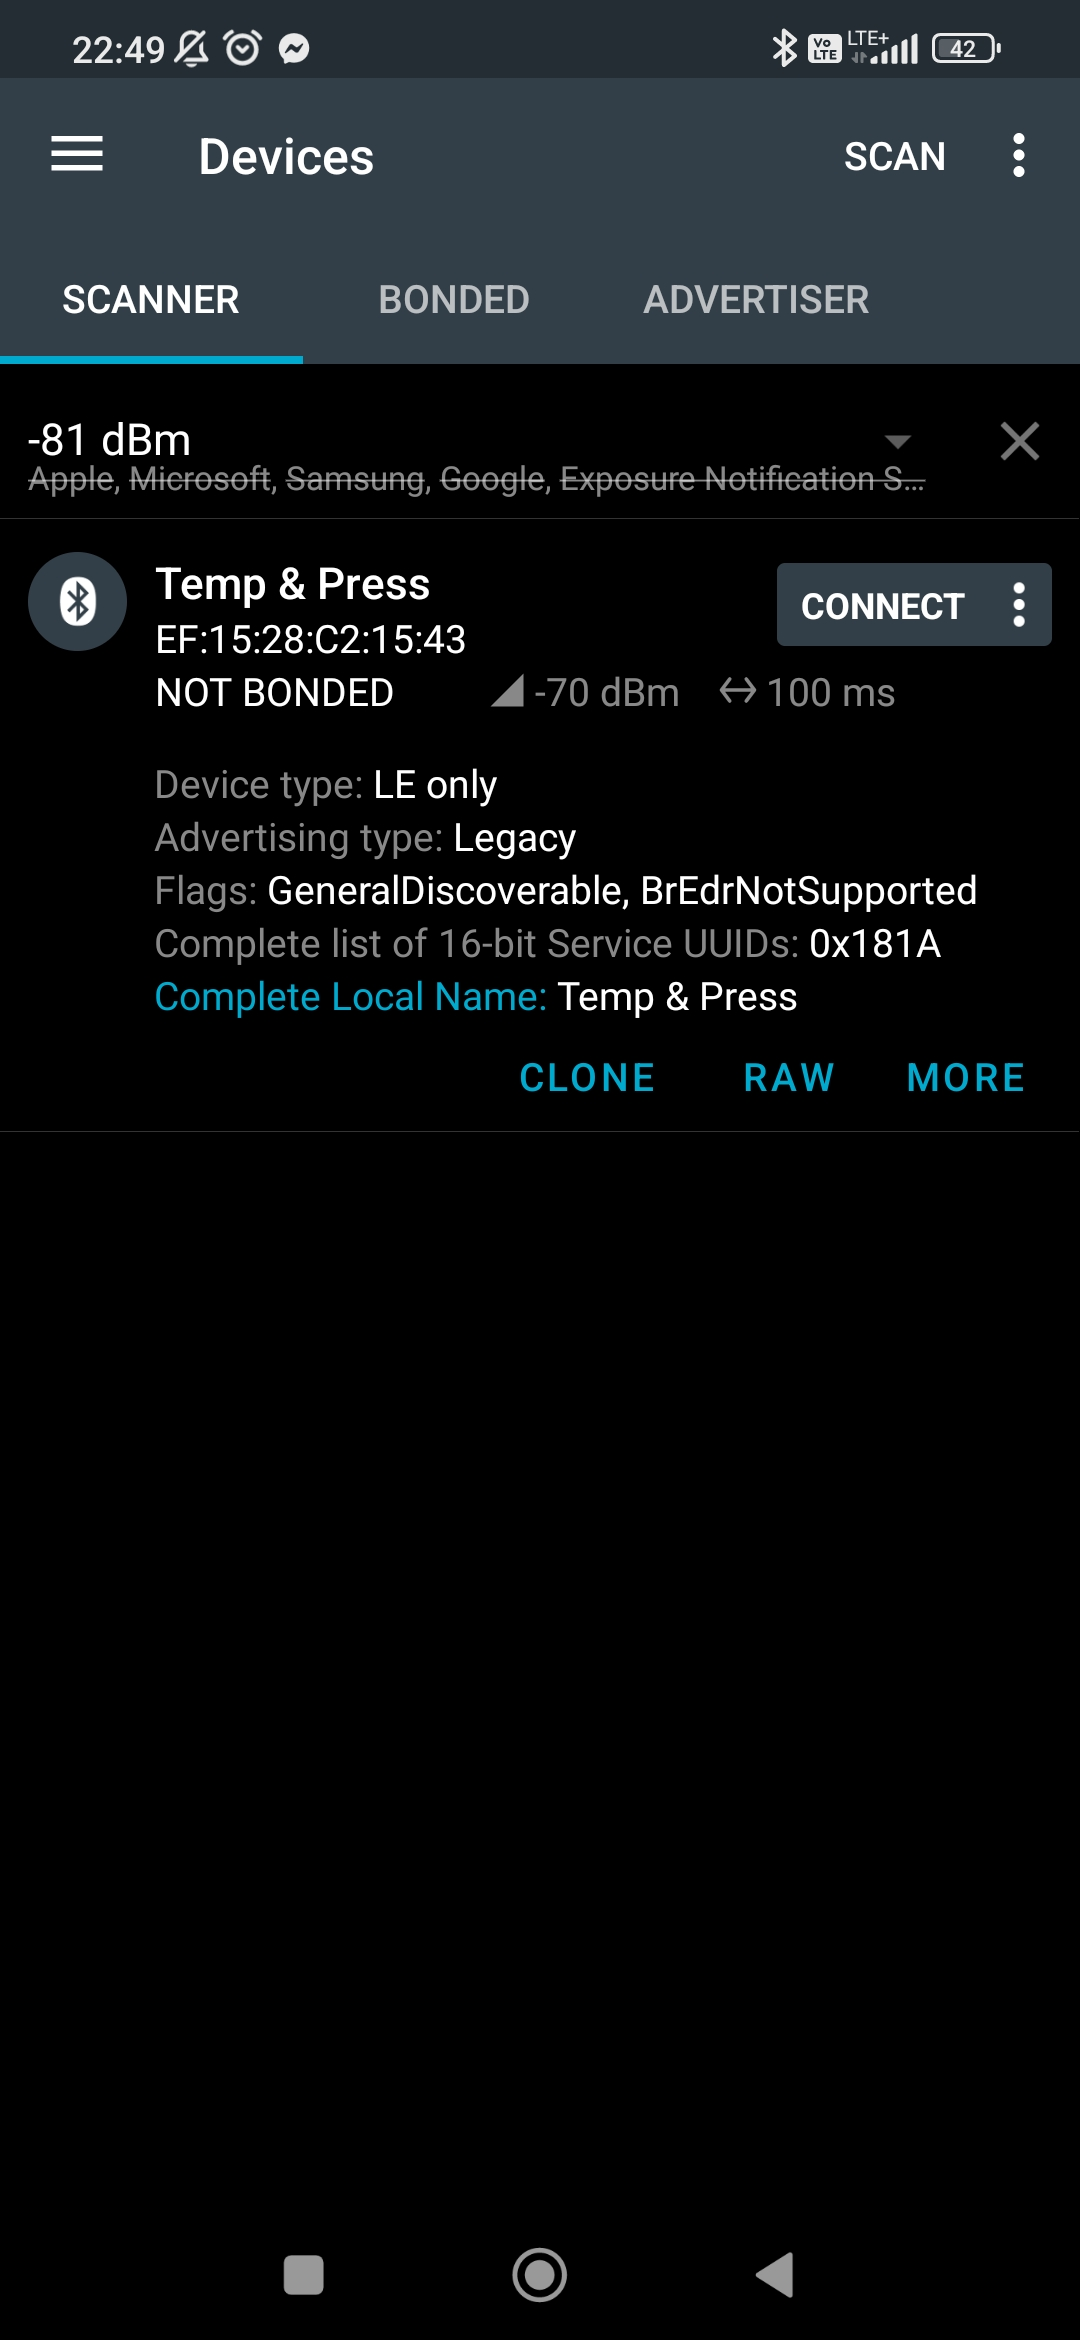
\includegraphics[scale=0.1]{nRFconnect_1}
\captionsetup{justification=centering}
\caption{Reklamowany serwis "Temp \& Press".}
\end{minipage}
\begin{minipage}[H]{0.4\textwidth}
\centering
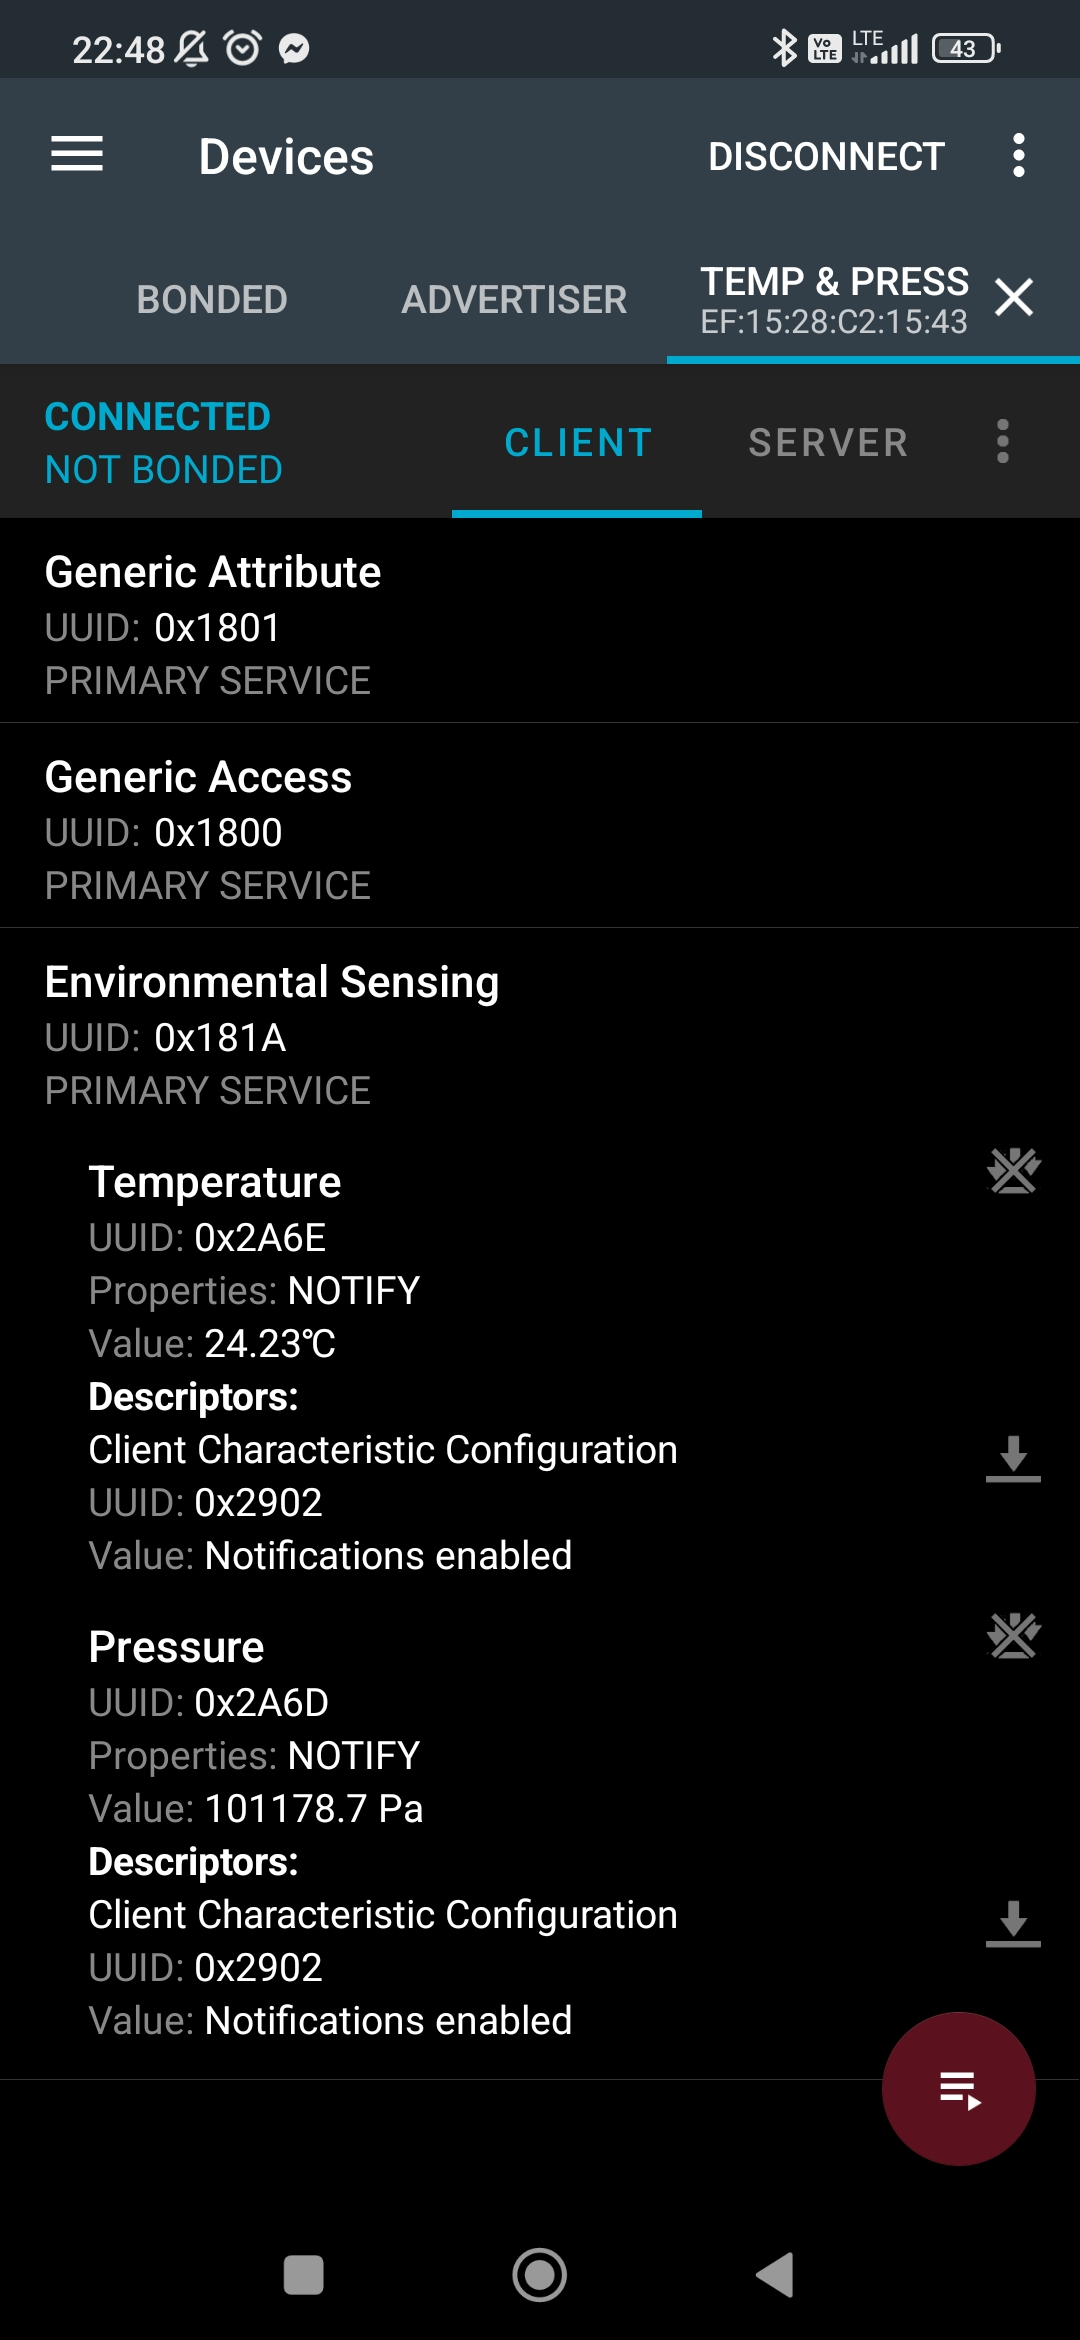
\includegraphics[scale=0.1]{nRFconnect_2}
\captionsetup{justification=centering}
\caption{Serwis po nawiązaniu połączenia.}
\end{minipage}
\end{figure}

Po podłączeniu Arduino 33 Nano BLE do zasilania płytka zaczyna nadawać reklamę serwisu pogodowego. Używając aplikacji mobilnej nRF Connect, zyskujemy dostęp do wszystkich urządzeń używających Bluetooth w zasięgu naszego telefonu. Na Rys.2. widzimy serwis reklamowany przez nasze Arduino. Po połączeniu się z serwerem przyciskiem "Connect", dostajemy dostęp do wszystkich szczegółów serwisów. Na Rys.3., w zakładce "Environmental Sensing" znajdują się pola reprezentujące aktualną temperaturę i ciśnienie atmosferyczne. Co każde 5 sekund Arduino wysyła pomiar z czujnika na połączony telefon.

\section{Fragmenty kodu}

\begin{figure}[H]
\centering
\includegraphics[scale=0.6]{definicja_reklamy}
\caption{Definicja reklamy dla serwisu.}
\end{figure}

\begin{figure}[H]
\centering
\includegraphics[scale=0.5]{definicja_serwisu}
\caption{Definicja serwisu.}
\end{figure}

\begin{figure}[H]
\centering
\includegraphics[scale=0.4]{main_1}
\caption{Inicjalizacja Bluetooth BLE i czujnika BMP280.}
\end{figure}

\begin{figure}[H]
\centering
\includegraphics[scale=0.4]{main_2}
\caption{Główna pętla.}
\end{figure}

\section{Kompilacja i flash'owanie}

\subsection{Budowanie projektu}

west build -p always -b arduino\_nano\_33\_ble \{ścieżka do projektu\}
\newline
\tab\tab-DDTC\_OVERLAY\_FILE="arduino\_i2c.overlay"

\subsection{Flash'owanie Arduino}
west flash --bossac=\{ścieżka do bossac.exe\} --bossac-port="COM3"


\end{document}
